% 0609/scan
\chapter{Mapping of camera coordinates onto LCoS coordinates}
\label{sec:rigid}
\begin{summary}
  In our microscope the plane of the camera is conjugate to the plane
  of the LCoS display. It is useful and for most illumination
  strategies crucial to be able to relate a camera position back to
  the LCoS. Then the information from one exposure can be used to
  control the illumination in the next.

  Whenever the camera is moved or the variable tubelens is changed, we
  have to recalibrate the system with a fluorescent plane sample on
  which we project single spots with known positions on the LCoS. Here
  we describe a robust approach to find a rigid transform between LCoS
  and camera coordinates.
\end{summary}
\section{Description of the rigid transform}
In order to relate coordinates on the LCoS display with pixel
positions on the camera, we found it suffices to use a rigid
transform. The rigid transform between display and camera is defined
as:
\begin{align}
  \r^d&=s \textrm{R}_\phi \r^c + \vect t\\
  \textrm{R}_\theta&=\begin{pmatrix}
  \cos\phi & q\sin\phi \\
  -\sin\phi & q\cos\phi \\ 
  \end{pmatrix}
\end{align}
where $\r^d$ is a point on the display, $\r^c$ is a point on the
camera and $q$ can be either $+1$ or $-1$. The value of $q$ is $-1$,
if there is a single axis reflection. It is $+1$ if there is no
reflection.

\begin{figure}[!hbt]
  \centering
  \input{calib-align.eps_tex}
  \caption{Given $n\ge 4$ camera images of a display showing one
    point.  It is possible to calculate the parameters of the rigid
    transform parameters scaling $s$, rotation angle $\phi$,
    translation vector $\vect t$.}
  \label{fig:calib-align}
\end{figure}



One can find the transform parameters scaling $s$, rotation angle
$\phi$, translation vector $\vect t$ by minimizing
\begin{align}
  \sum_i^n \abs{s \textrm{R}_\phi \r^c_i+\vect t -\r^d_i}^2 \label{eq:rigid-sum}
\end{align}
for all $n$ points on the display $\r^d_i$ and there corresponding
camera positions $\r^c_i$.  Each term of the sum can be expressed as
two scalar terms:
\begin{align*}
  \sum_i^n&
  \abs{s(\cos\phi r^c_{ix}+q\sin\phi r^c_{iy})+t_x-r^d_{ix}}^2
  +
  \abs{s(-\sin\phi r^c_{ix}+q\cos\phi r^c_{iy})+t_y-r^d_{iy}}^2
\end{align*}

The following Maxima code will find the solution to the least squares
problem:
\begin{verbatim}
load(minpack)$
q:-1;
g(s,p,tx,ty):=[s*( cos(p)*<cx>+q*sin(p)*<cy>)+tx-<dx>,
               s*(-sin(p)*<cx>+q*cos(p)*<cy>)+ty-<dy>, ... ]$
minpack_lsquares(g(s,p,tx,ty), [s,p,tx,ty], [0.88,-3.1,1200,-20]);
\end{verbatim}
We define the function \verb!g! to contain all the terms of the sum.
This can easily written by a program that constructs the lines
according to the given pattern, replacing \verb!<cx>!, \verb!<cy>!
with camera coordinates and \verb!<dx>!, \verb!<dy>! with display
coordinates.

The function \verb!minpack_lsquares! calls the subroutine \verb!lmder!
which was originally developed for the Fortran\footnote{Rather than
  calling a Fortran library Maxima calls a version of this function
  that was automatically translated into Common Lisp via {\sf f2cl}.}
package \verb!minpack!.

{\small
\begin{verbatim}
c     subroutine lmder (http://www.netlib.org/minpack/lmder.f)
c     the purpose of lmder is to minimize the sum of the squares of
c     m nonlinear functions in n variables by a modification of
c     the levenberg-marquardt algorithm. the user must provide a
c     subroutine which calculates the functions and the jacobian.
c     the subroutine statement is
c       subroutine lmder(fcn,m,n,x,fvec,fjac,ldfjac,ftol,xtol,gtol,
c                        maxfev,diag,mode,factor,nprint,info,nfev,
c                        njev,ipvt,qtf,wa1,wa2,wa3,wa4)
\end{verbatim}
}

\noindent The reason for using Maxima is, that it calculates the symbolic
Jacobian for the problem. This makes it straight forward to change the
simple rigid transform to a model with more parameters.

The following Common Lisp code shows how the result of the
optimization can be used to initialize the OpenGL modelview matrix to
transform objects in its buffer, so that they will appear at the given
positions on the camera.

{\small
\begin{verbatim}
(defun load-cam-to-lcos-matrix (&optional (x 0s0) (y 0s0))
  (let* ((s 0.828333873909549) (sx  s)        (sy  (- s))
         (phi -3.102)          (sp (sin phi)) (cp (cos phi))
         (tx 608.433)          (ty 168.918)
         (a (make-array (list 4 4) :element-type 'single-float
             :initial-contents
             (list (list (* sx cp)    (* sy sp)  .0   (+ x tx))
                   (list (* -1 sx sp) (* sy cp)  .0   (+ y ty))
                   (list .0           .0        1.0   .0)
                   (list .0           .0         .0  1.0)))))
    (gl:load-transpose-matrix (sb-ext:array-storage-vector a))))    
\end{verbatim}
}
  

\noindent
Alternatively, here is the equivalent code in C:

{\small
\begin{verbatim}
float m[4*4]; // OpenGL Modelview Matrix
float s=-.8749328910202312,
      sx=s,sy=-s,phi=-.8052030670943575,
      cp=cos(phi),sp=sin(phi),
      tx=1456.71806436377,
      ty=910.4787738693659;
  m[0]=   sx*cp;   m[4]=sy*sp;   m[8] =0;    m[12]=tx; 
  m[1]=-1*sx*sp;   m[5]=sy*cp;   m[9] =0;    m[13]=ty; 
  m[2]=0;          m[6]=0.;      m[10]=1;    m[14]=0;  
  m[3]=0;          m[7]=0.;      m[11]=0;    m[15]=1;  
glMatrixMode(GL_MODELVIEW);
glLoadMatrixf(m);
\end{verbatim}
}
\section{Experimental example and image processing}

For the calibration a fluorescent plane (see
\figref{fig:rigid-pics}~left for a uniform wide field image) is imaged
with the LCoS display showing spots in the illuminated area.  Ideally
for this measurement all mirrors on the MMA are undeflected and the
apertures $B_0$ and $B_1$ completely open (see
\figref{fig:memi-real}). Then the square exit of the integrating
tunnel illuminates the biggest possible area on the LCoS.

\begin{figure}[!hbt]
  \centering
  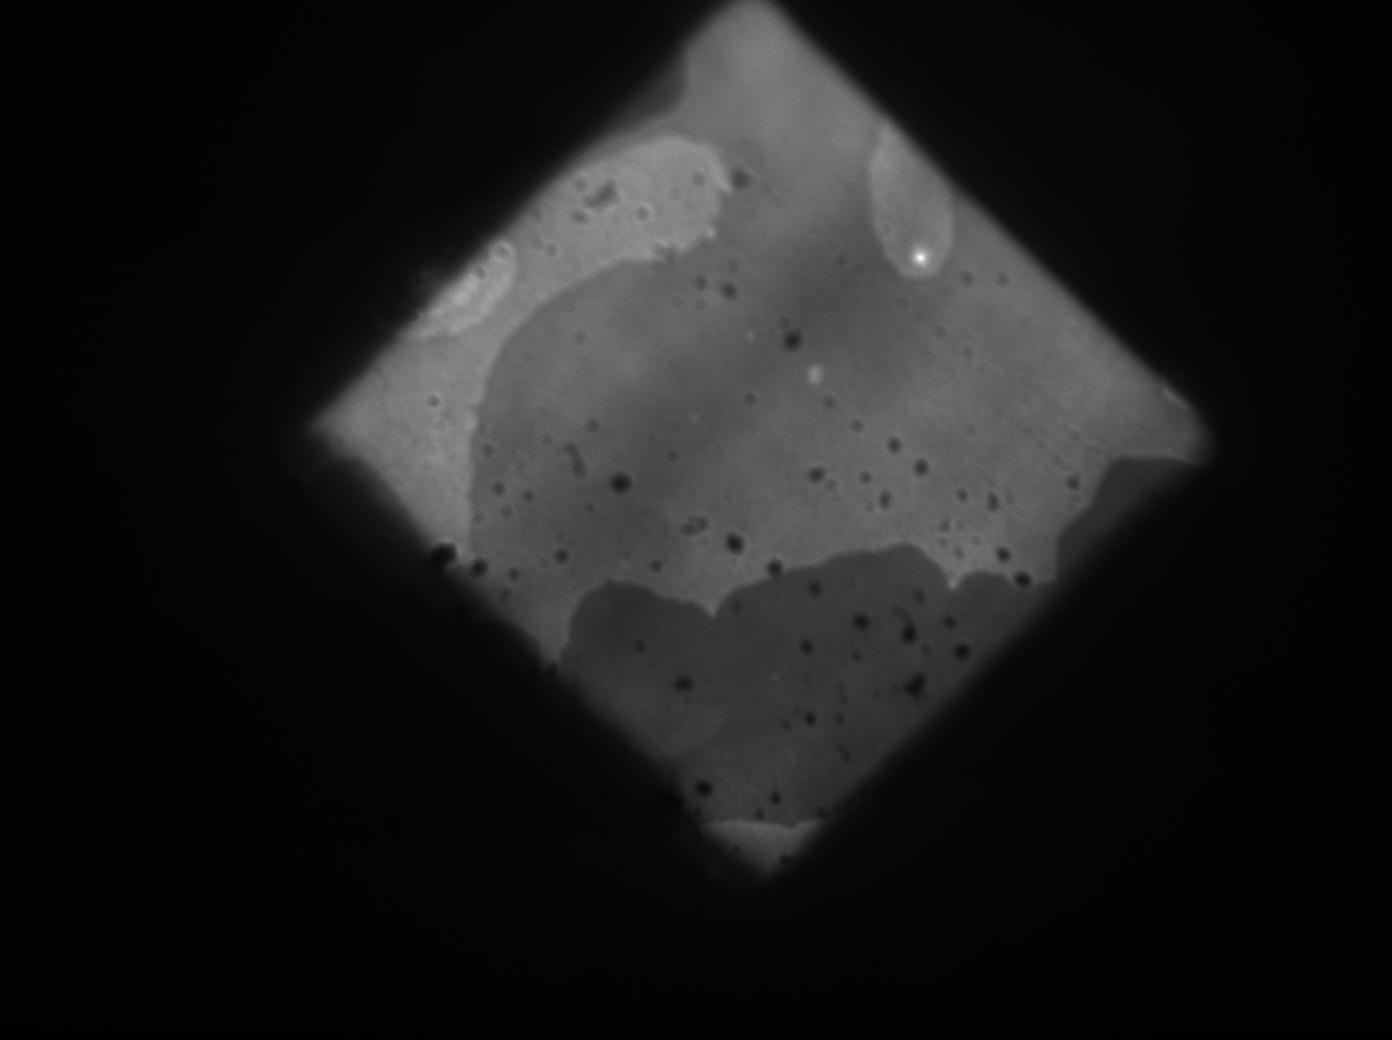
\includegraphics[width=7cm]{o102}
  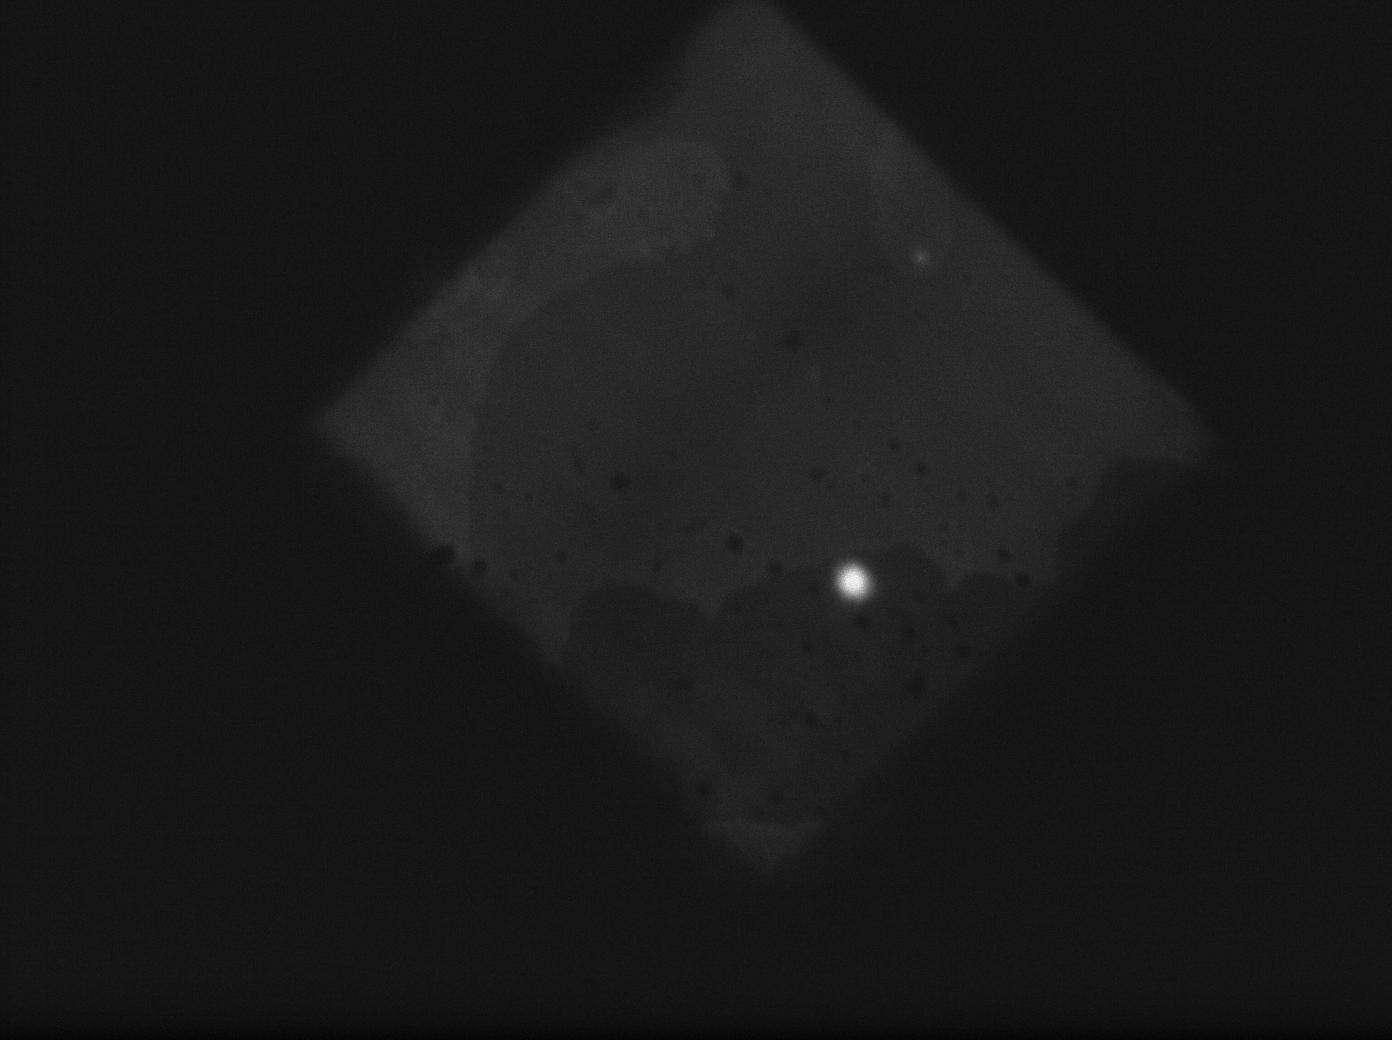
\includegraphics[width=7cm]{o035}
  \caption{{\bf left:} Uniformly illuminated fluorescent plane (mono
    and double layer of yellow beads with \unit[110]{nm} diameter,
    excited with \unit[473]{nm} laser in a 63x/1.47 objective). {\bf
      right:} Image with the the LCoS displaying a disk with 24 pixels
    diameter (corresponding to $\unit[2.4]{\mu m}$ in the sample)
    centred at LCoS position $(550,750)$.}
  \label{fig:rigid-pics}
\end{figure}

% i believe the TL_ill is set to r_MMA=3.84mm in BFP 
% f_TLill = 352 mm
% mag_real = mag / f_zeiss * f_TLill 
% pixel-pitch-lcos / mag_real
% one pixel is: 13.62 / 63 * 164.5 / 352 = 101nm

\begin{figure}[!hbt]
  \centering
  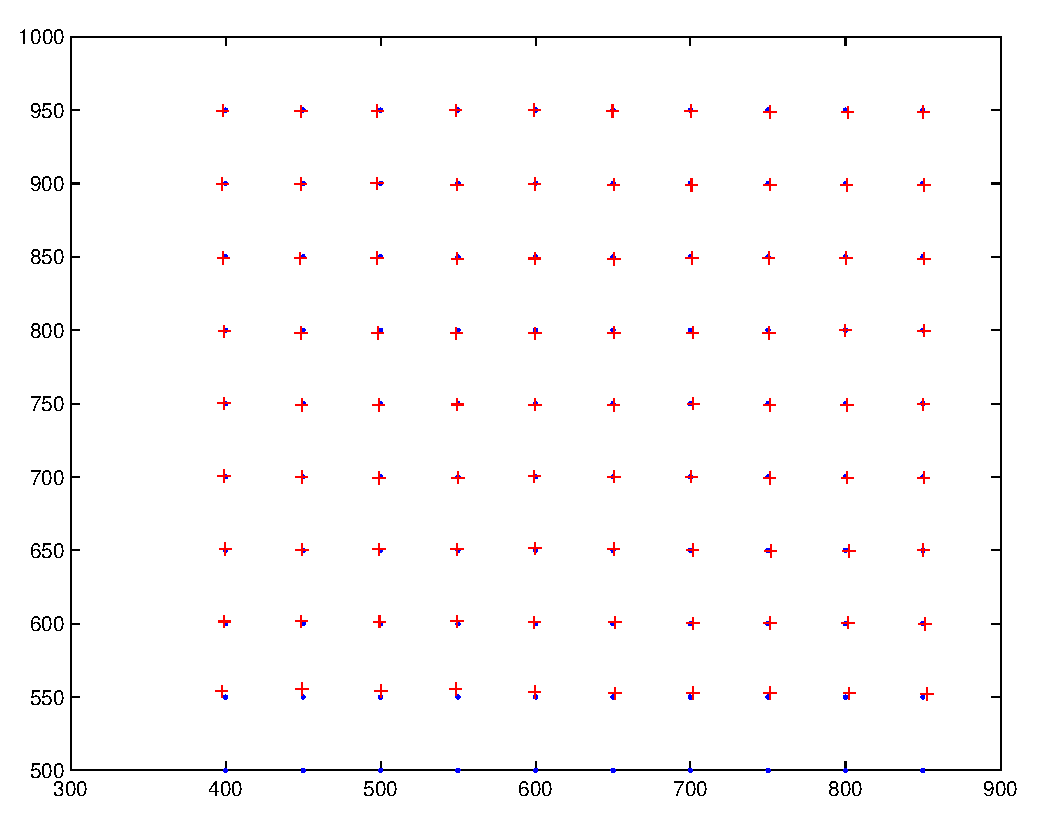
\includegraphics[width=12cm]{../rigid/rigid-compare}
  \caption{Red ``$+$'' signs indicate where the spots that were
    localized in the camera images end up after a rigid
    transform. There is sufficient agreement with the original
    display positions.}
  \label{fig:rigid-compare}
\end{figure}

For the calibration $10\times10$ images (100 images, each containing
one bright spot at a different position) were captured with a disk of
24 pixels diameter at the positions $(400+50i,500+50j)\ \forall i,j\in
[0,99]$. Furthermore, one uniformly illuminated image is used to
correct for intensity fluctuations in the fluorescent plane.  The
following Matlab/DIPimage code is used to normalize the images and
localize the spots. The coordinates are then assembled into the Maxima
command that finds the parameters of the rigid transform. Finally the
transformed spot positions from the camera images are compared with
the original LCoS pixel positions.

The following Matlab listing shows how to open the image files:
% cd /mnt/scan 
{\small
\begin{verbatim}
%% load the files
% 0 .. 99 spot images
% only 10..99 usable because the first are on border and not illuminated
a = newim(1392,1040,103);
for i=0:102
    % Andor's FITS format isn't read correctly
    % correct this by adding 2^15
    a(:,:,i) = 2^15 + readim(sprintf('o%03d.fits',i));
end
\end{verbatim}}

  Of the 103 images, that are loaded into \verb!a!, the first 100
  contain spots and the image at the zero-based index 102 is the
  uniformly illuminated image shown in \figref{fig:rigid-pics} left.
  The other two images at indices 100 and 101 are two centered disks
  with different diameters and are not used here.

{\small
\begin{verbatim}
bright = squeeze(a(:,:,102));  % histogram of uniformly illuminated
                               % image has minimum at 800 ADU
mask = gaussf(bright,8) > 800; % create mask with illuminated area
bg = 510;                      % the background is be 510 ADU

posmax = newim(100,2);
for i = 10:99
    % correct for sample non-uniformity 
    corr = (squeeze(a(:,:,i)) - bg) / bright * mask;
    % find coordinates of maximum
    [coords,vals]=findmaxima(gaussf(corr,32));
    [valss,valsind] = sort(vals);   % sort coordinates by intensity
    tmp = coords(valsind,:);        % collect the maximum with highest
    posmax(i,:) = tmp(end,:);       % intensity into result
end
\end{verbatim}}
  
  The DIPimage toolbox provides the function \verb!findmaxima!, that
  locates all local maxima in an image with subpixel accurac y. We
  sort the result by gray value and only use the biggest.  The
  measured 100 camera coordinate pairs in \verb!posmax! correspond to
  $\r^c_i$ in equation \ref{eq:rigid-sum}.
 
  From Matlab we create the file \verb!fit.max! with batch commands
  for Maxima. Then we run Maxima. When it is finished after a few
  seconds, the file \verb!max.out! will contain the four fitted
  parameters.
 
{\small
\begin{verbatim}
c = double(posmax)';
cmd = '';                       % collect equations in maxima format
for i=10:99
    dx = num2str(400+50*mod(i,10));
    dy = num2str(500+50*floor(i./10));
    cx = num2str(c(i+1,1)); 
    cy = num2str(c(i+1,2));
    cmd=[cmd ' s*( cos(p)*' cx '+q*sin(p)*' cy ')+tx-' dx ', ...
         s*(-sin(p)*'cx '+q*cos(p)*' cy ')+ty-' dy ','];
end
cmd(:,end) = []; % delete last comma

% load the fitting package and start defining the merit function g
pre = 'load(minpack)$ q:-1; g(s,p,tx,ty):=[';
% now put cmd between
% call the fitting function and store the parameters into max.out
cod = [']$ fit:minpack_lsquares(g(s,p,x,y),[s,p,x,y],[.88,-1.3,1200,-20]);' ...
 'write_data(fit[1],"max.out");']

fid = fopen('fit.max','w'); % write maxima commands into file 
fwrite(fid,[pre cmd cod]);
fclose(fid);
[max_status,max_result]=system('maxima -b fit.max');  % execute maxima
\end{verbatim}}

  We load the transformation parameters back into Matlab and create
  the diagram \figref{fig:rigid-compare} to visualize, how well the
  transform matches camera and display coordinates.

{\small
\begin{verbatim}
% load rigid transformation parameters from the file into matlab
params = load('max.out')'; 
scale = params(1); phi = params(2);
tx = params(3);    ty = params(4);

mirr = -1;
R = [cos(phi),mirr*sin(phi);
     -sin(phi),mirr*cos(phi)];
T = [tx ty]';

%% plot the two grids on top of each other
mapped = zeros(100,2);
for i=11:100 % camera coordinates into display coordinates
    mapped(i,:) = (scale*R*q(i,:)'+T)';
end

dpos = zeros(100,2);
for i=0:99 % calculate display points
    dpos(i+1,1) = 400+50*mod(i,10);
    dpos(i+1,2) = 500+50*floor(i./10);
end

hold off;  plot(dpos(:,1),dpos(:,2),'.');
hold on;   plot(mapped(11:end,1),mapped(11:end,2),'r+');
\end{verbatim}}
% print -depsc2 /home/martin/thesis/kielhorn/rigid/rigid-compare

\section{Conclusion}
The rigid transform and our method to estimate its parameters is a
sufficient and robust method, to map the coordinates of our camera
into those of the spatial display.

The rigid transform can be done directly in OpenGL. Hence, it is
trivial to render a properly transformed texture of the camera
image which is then shown on the display.

An advantage over other methods, e.g. finding a homology matrix via
RANSAC, is that the result is not a transformation matrix but
separated parameters for scaling, rotation and translation. 